\documentclass{standalone}
\usepackage{tikz}
\usetikzlibrary{patterns, positioning}

\begin{document}
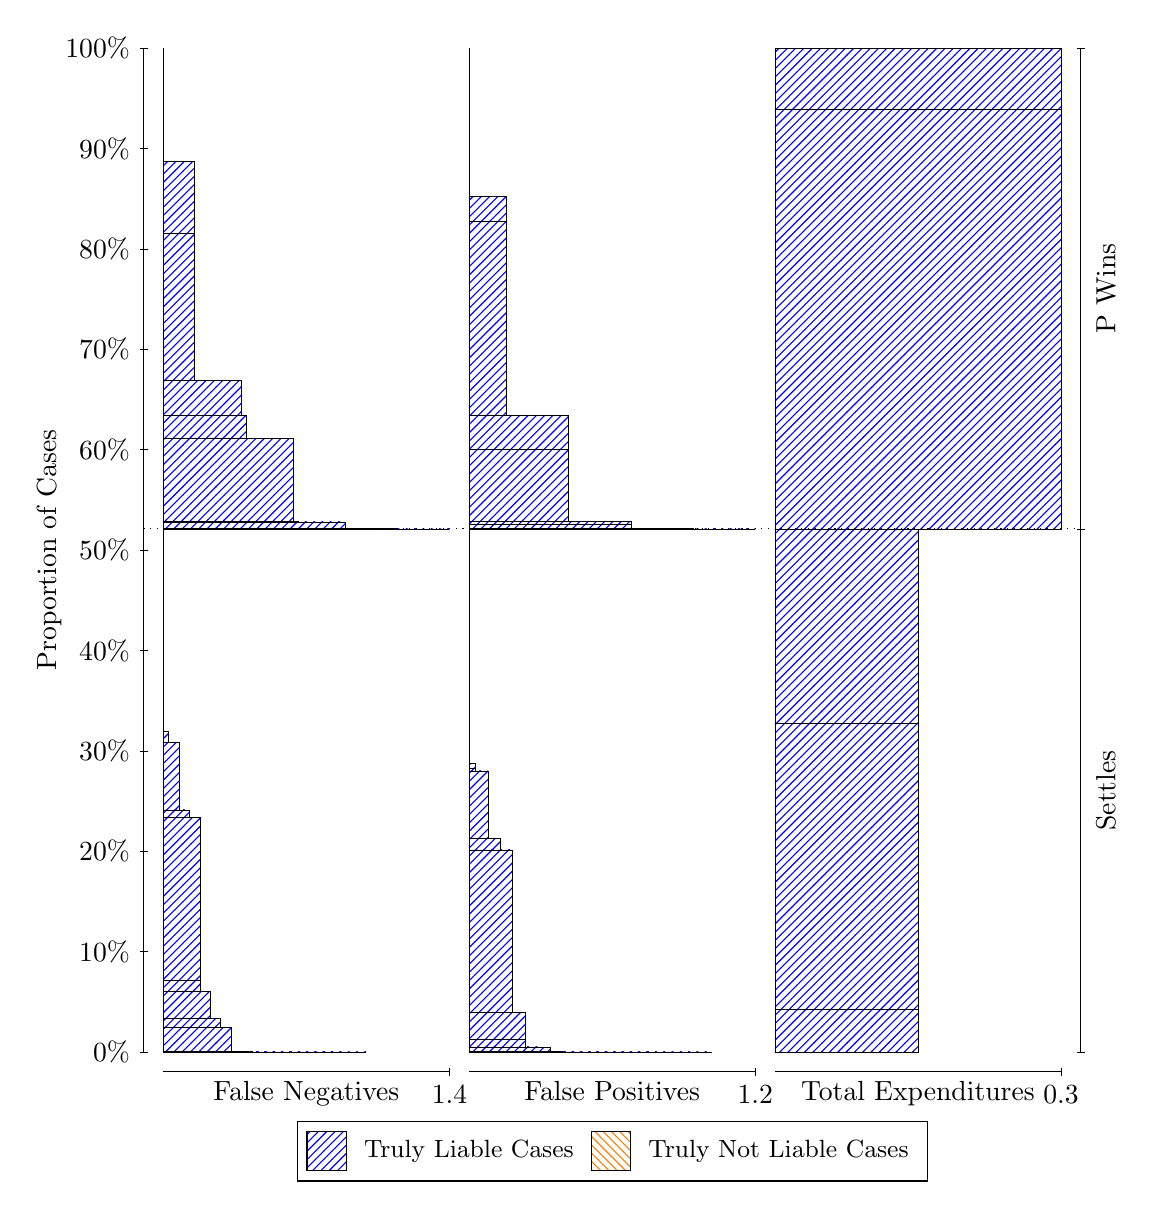
\begin{tikzpicture}
\draw[black, very thin] (1.5,1.75) -- (1.5,14.5);
\node[rotate=90, anchor=center] at (0.3, 8.125) {Proportion of Cases};
\draw[black, very thin] (1.45,1.75) -- (1.55,1.75);
\node[anchor=east] at (1.45, 1.75) {0\%};
\draw[black, very thin] (1.45,3.025) -- (1.55,3.025);
\node[anchor=east] at (1.45, 3.025) {10\%};
\draw[black, very thin] (1.45,4.3) -- (1.55,4.3);
\node[anchor=east] at (1.45, 4.3) {20\%};
\draw[black, very thin] (1.45,5.575) -- (1.55,5.575);
\node[anchor=east] at (1.45, 5.575) {30\%};
\draw[black, very thin] (1.45,6.85) -- (1.55,6.85);
\node[anchor=east] at (1.45, 6.85) {40\%};
\draw[black, very thin] (1.45,8.125) -- (1.55,8.125);
\node[anchor=east] at (1.45, 8.125) {50\%};
\draw[black, very thin] (1.45,9.4) -- (1.55,9.4);
\node[anchor=east] at (1.45, 9.4) {60\%};
\draw[black, very thin] (1.45,10.675) -- (1.55,10.675);
\node[anchor=east] at (1.45, 10.675) {70\%};
\draw[black, very thin] (1.45,11.95) -- (1.55,11.95);
\node[anchor=east] at (1.45, 11.95) {80\%};
\draw[black, very thin] (1.45,13.225) -- (1.55,13.225);
\node[anchor=east] at (1.45, 13.225) {90\%};
\draw[black, very thin] (1.45,14.5) -- (1.55,14.5);
\node[anchor=east] at (1.45, 14.5) {100\%};

\draw[black, very thin] (13.4,1.75) -- (13.4,14.5);
\draw[black, very thin] (13.35,1.75) -- (13.45,1.75);
\node[anchor=west] at (13.35, 1.75) {};
\draw[black, very thin] (13.35,8.3942) -- (13.45,8.3942);
\node[anchor=west] at (13.35, 8.3942) {};
\draw[black, very thin] (13.35,14.5) -- (13.45,14.5);
\node[anchor=west] at (13.35, 14.5) {};

\draw[black, very thin, pattern color=blue, pattern=north east lines] (1.75,1.75) rectangle (4.3264,1.75);
\draw[black, very thin, pattern color=blue, pattern=north east lines] (1.75,1.75) rectangle (4.0621,1.75);
\draw[black, very thin, pattern color=blue, pattern=north east lines] (1.75,1.75) rectangle (3.7979,1.75);
\draw[black, very thin, pattern color=blue, pattern=north east lines] (1.75,1.75) rectangle (3.6658,1.75);
\draw[black, very thin, pattern color=blue, pattern=north east lines] (1.75,1.75) rectangle (3.5336,1.75);
\draw[black, very thin, pattern color=blue, pattern=north east lines] (1.75,1.75) rectangle (3.4015,1.75);
\draw[black, very thin, pattern color=blue, pattern=north east lines] (1.75,1.75) rectangle (3.2694,1.7508);
\draw[black, very thin, pattern color=blue, pattern=north east lines] (1.75,1.7508) rectangle (3.1373,1.751);
\draw[black, very thin, pattern color=blue, pattern=north east lines] (1.75,1.751) rectangle (3.0052,1.7515);
\draw[black, very thin, pattern color=blue, pattern=north east lines] (1.75,1.7515) rectangle (2.873,1.7535);
\draw[black, very thin, pattern color=blue, pattern=north east lines] (1.75,1.7535) rectangle (2.7409,1.7581);
\draw[black, very thin, pattern color=blue, pattern=north east lines] (1.75,1.7581) rectangle (2.6088,2.0621);
\draw[black, very thin, pattern color=blue, pattern=north east lines] (1.75,2.0621) rectangle (2.4767,2.1786);
\draw[black, very thin, pattern color=blue, pattern=north east lines] (1.75,2.1786) rectangle (2.3445,2.5169);
\draw[black, very thin, pattern color=blue, pattern=north east lines] (1.75,2.5169) rectangle (2.2124,2.6612);
\draw[black, very thin, pattern color=blue, pattern=north east lines] (1.75,2.6612) rectangle (2.2124,4.727);
\draw[black, very thin, pattern color=blue, pattern=north east lines] (1.75,4.727) rectangle (2.0803,4.8249);
\draw[black, very thin, pattern color=blue, pattern=north east lines] (1.75,4.8249) rectangle (1.9482,5.6821);
\draw[black, very thin, pattern color=blue, pattern=north east lines] (1.75,5.6821) rectangle (1.8161,5.8267);
\draw[black, very thin, pattern color=orange, pattern=north west lines] (1.75,5.8267) rectangle (1.75,5.8267);
\draw[black, very thin, pattern color=blue, pattern=north east lines] (1.75,5.8267) rectangle (1.75,8.3942);
\draw[black, very thin, pattern color=blue, pattern=north east lines] (1.75,8.3942) rectangle (5.3833,8.3942);
\draw[black, very thin, pattern color=blue, pattern=north east lines] (1.75,8.3942) rectangle (4.7227,8.3953);
\draw[black, very thin, pattern color=blue, pattern=north east lines] (1.75,8.3953) rectangle (4.1282,8.3953);
\draw[black, very thin, pattern color=blue, pattern=north east lines] (1.75,8.3953) rectangle (4.0621,8.4834);
\draw[black, very thin, pattern color=blue, pattern=north east lines] (1.75,8.4834) rectangle (3.4676,8.4836);
\draw[black, very thin, pattern color=blue, pattern=north east lines] (1.75,8.4836) rectangle (3.4015,9.5407);
\draw[black, very thin, pattern color=blue, pattern=north east lines] (1.75,9.5407) rectangle (2.807,9.8334);
\draw[black, very thin, pattern color=blue, pattern=north east lines] (1.75,9.8334) rectangle (2.7409,10.28);
\draw[black, very thin, pattern color=blue, pattern=north east lines] (1.75,10.28) rectangle (2.1464,12.145);
\draw[black, very thin, pattern color=blue, pattern=north east lines] (1.75,12.145) rectangle (2.1464,13.06);
\draw[black, very thin, pattern color=blue, pattern=north east lines] (1.75,13.06) rectangle (2.0803,13.06);
\draw[black, very thin, pattern color=orange, pattern=north west lines] (1.75,13.06) rectangle (1.75,13.06);
\draw[black, very thin, pattern color=blue, pattern=north east lines] (1.75,13.06) rectangle (1.75,14.5);
\draw[black, very thin, pattern color=orange, pattern=north west lines] (5.6333,1.75) rectangle (8.7138,1.75);
\draw[black, very thin, pattern color=blue, pattern=north east lines] (5.6333,1.75) rectangle (8.7138,1.75);
\draw[black, very thin, pattern color=orange, pattern=north west lines] (5.6333,1.75) rectangle (8.0819,1.75);
\draw[black, very thin, pattern color=blue, pattern=north east lines] (5.6333,1.75) rectangle (8.0819,1.75);
\draw[black, very thin, pattern color=blue, pattern=north east lines] (5.6333,1.75) rectangle (7.9239,1.75);
\draw[black, very thin, pattern color=orange, pattern=north west lines] (5.6333,1.75) rectangle (7.7659,1.75);
\draw[black, very thin, pattern color=blue, pattern=north east lines] (5.6333,1.75) rectangle (7.7659,1.75);
\draw[black, very thin, pattern color=orange, pattern=north west lines] (5.6333,1.75) rectangle (7.45,1.75);
\draw[black, very thin, pattern color=blue, pattern=north east lines] (5.6333,1.75) rectangle (7.45,1.7501);
\draw[black, very thin, pattern color=blue, pattern=north east lines] (5.6333,1.7501) rectangle (7.292,1.7501);
\draw[black, very thin, pattern color=orange, pattern=north west lines] (5.6333,1.7501) rectangle (7.1341,1.7501);
\draw[black, very thin, pattern color=blue, pattern=north east lines] (5.6333,1.7501) rectangle (7.1341,1.7504);
\draw[black, very thin, pattern color=blue, pattern=north east lines] (5.6333,1.7504) rectangle (7.1341,1.7509);
\draw[black, very thin, pattern color=blue, pattern=north east lines] (5.6333,1.7509) rectangle (6.9761,1.7509);
\draw[black, very thin, pattern color=orange, pattern=north west lines] (5.6333,1.7509) rectangle (6.8181,1.7509);
\draw[black, very thin, pattern color=blue, pattern=north east lines] (5.6333,1.7509) rectangle (6.8181,1.7527);
\draw[black, very thin, pattern color=blue, pattern=north east lines] (5.6333,1.7527) rectangle (6.6601,1.8114);
\draw[black, very thin, pattern color=orange, pattern=north west lines] (5.6333,1.8114) rectangle (6.5022,1.8114);
\draw[black, very thin, pattern color=blue, pattern=north east lines] (5.6333,1.8114) rectangle (6.5022,1.8132);
\draw[black, very thin, pattern color=blue, pattern=north east lines] (5.6333,1.8132) rectangle (6.5022,1.8156);
\draw[black, very thin, pattern color=blue, pattern=north east lines] (5.6333,1.8156) rectangle (6.3442,1.9135);
\draw[black, very thin, pattern color=blue, pattern=north east lines] (5.6333,1.9135) rectangle (6.3442,2.2513);
\draw[black, very thin, pattern color=orange, pattern=north west lines] (5.6333,2.2513) rectangle (6.1862,2.2513);
\draw[black, very thin, pattern color=blue, pattern=north east lines] (5.6333,2.2513) rectangle (6.1862,4.3171);
\draw[black, very thin, pattern color=blue, pattern=north east lines] (5.6333,4.3171) rectangle (6.1862,4.3175);
\draw[black, very thin, pattern color=blue, pattern=north east lines] (5.6333,4.3175) rectangle (6.0283,4.4621);
\draw[black, very thin, pattern color=blue, pattern=north east lines] (5.6333,4.4621) rectangle (5.8703,5.3193);
\draw[black, very thin, pattern color=blue, pattern=north east lines] (5.6333,5.3193) rectangle (5.7123,5.3538);
\draw[black, very thin, pattern color=blue, pattern=north east lines] (5.6333,5.3538) rectangle (5.7123,5.4172);
\draw[black, very thin, pattern color=blue, pattern=north east lines] (5.6333,5.4172) rectangle (5.6333,8.3942);
\draw[black, very thin, pattern color=orange, pattern=north west lines] (5.6333,8.3942) rectangle (9.2667,8.3942);
\draw[black, very thin, pattern color=blue, pattern=north east lines] (5.6333,8.3942) rectangle (9.2667,8.3942);
\draw[black, very thin, pattern color=orange, pattern=north west lines] (5.6333,8.3942) rectangle (8.4768,8.3942);
\draw[black, very thin, pattern color=blue, pattern=north east lines] (5.6333,8.3942) rectangle (8.4768,8.3945);
\draw[black, very thin, pattern color=blue, pattern=north east lines] (5.6333,8.3945) rectangle (8.4768,8.3953);
\draw[black, very thin, pattern color=orange, pattern=north west lines] (5.6333,8.3953) rectangle (7.687,8.3953);
\draw[black, very thin, pattern color=blue, pattern=north east lines] (5.6333,8.3953) rectangle (7.687,8.4525);
\draw[black, very thin, pattern color=blue, pattern=north east lines] (5.6333,8.4525) rectangle (7.687,8.4844);
\draw[black, very thin, pattern color=orange, pattern=north west lines] (5.6333,8.4844) rectangle (6.9761,8.4844);
\draw[black, very thin, pattern color=blue, pattern=north east lines] (5.6333,8.4844) rectangle (6.9761,8.4844);
\draw[black, very thin, pattern color=orange, pattern=north west lines] (5.6333,8.4844) rectangle (6.8971,8.4844);
\draw[black, very thin, pattern color=blue, pattern=north east lines] (5.6333,8.4844) rectangle (6.8971,9.4011);
\draw[black, very thin, pattern color=blue, pattern=north east lines] (5.6333,9.4011) rectangle (6.8971,9.8342);
\draw[black, very thin, pattern color=blue, pattern=north east lines] (5.6333,9.8342) rectangle (6.1862,9.8342);
\draw[black, very thin, pattern color=orange, pattern=north west lines] (5.6333,9.8342) rectangle (6.1862,9.8342);
\draw[black, very thin, pattern color=blue, pattern=north east lines] (5.6333,9.8342) rectangle (6.1862,9.8343);
\draw[black, very thin, pattern color=blue, pattern=north east lines] (5.6333,9.8343) rectangle (6.1072,12.296);
\draw[black, very thin, pattern color=blue, pattern=north east lines] (5.6333,12.296) rectangle (6.1072,12.614);
\draw[black, very thin, pattern color=orange, pattern=north west lines] (5.6333,12.614) rectangle (5.6333,12.614);
\draw[black, very thin, pattern color=blue, pattern=north east lines] (5.6333,12.614) rectangle (5.6333,14.5);
\draw[black, very thin, pattern color=orange, pattern=north west lines] (9.5167,1.75) rectangle (11.333,1.75);
\draw[black, very thin, pattern color=blue, pattern=north east lines] (9.5167,1.75) rectangle (11.333,2.2951);
\draw[black, very thin, pattern color=orange, pattern=north west lines] (9.5167,2.2951) rectangle (11.333,2.2951);
\draw[black, very thin, pattern color=blue, pattern=north east lines] (9.5167,2.2951) rectangle (11.333,5.92);
\draw[black, very thin, pattern color=orange, pattern=north west lines] (9.5167,5.92) rectangle (11.333,5.92);
\draw[black, very thin, pattern color=blue, pattern=north east lines] (9.5167,5.92) rectangle (11.333,8.3942);
\draw[black, very thin, pattern color=orange, pattern=north west lines] (9.5167,8.3942) rectangle (13.15,8.3942);
\draw[black, very thin, pattern color=blue, pattern=north east lines] (9.5167,8.3942) rectangle (13.15,13.716);
\draw[black, very thin, pattern color=orange, pattern=north west lines] (9.5167,13.716) rectangle (13.15,13.716);
\draw[black, very thin, pattern color=blue, pattern=north east lines] (9.5167,13.716) rectangle (13.15,14.5);
\draw[black, dotted] (1.5,8.3942) -- (13.4,8.3942);
\draw[black, very thin] (1.75,1.5) -- (5.3833,1.5);
\node[anchor=north] at (3.5667, 1.5) {False Negatives};
\draw[black, very thin] (5.3833,1.45) -- (5.3833,1.55);
\node[anchor=north] at (5.3833, 1.45) {1.4};

\draw[black, very thin] (5.6333,1.5) -- (9.2667,1.5);
\node[anchor=north] at (7.45, 1.5) {False Positives};
\draw[black, very thin] (9.2667,1.45) -- (9.2667,1.55);
\node[anchor=north] at (9.2667, 1.45) {1.2};

\draw[black, very thin] (9.5167,1.5) -- (13.15,1.5);
\node[anchor=north] at (11.333, 1.5) {Total Expenditures};
\draw[black, very thin] (13.15,1.45) -- (13.15,1.55);
\node[anchor=north] at (13.15, 1.45) {0.3};

\node[black, centered, rotate=90] at (13.72, 5.0721) {Settles};
\node[black, centered, rotate=90] at (13.72, 11.447) {P Wins};

\draw (7.449999999999999,1.5) node[draw=none] (baseCoordinate) {};
\begin{scope}[align=center]
        \matrix[scale=0.5, draw=black, below=0.5cm of baseCoordinate, nodes={draw}, column sep=0.1cm]{
            \node[rectangle, draw, minimum width=0.5cm, minimum height=0.5cm, pattern=north east lines, pattern color=blue] {}; &
            \node[draw=none, font=\small] (B) {Truly Liable Cases}; &
            \node[rectangle, draw, minimum width=0.5cm, minimum height=0.5cm, pattern=north west lines, pattern color=orange] {}; &
            \node[draw=none, font=\small] (B) {Truly Not Liable Cases}; \\
            };
\end{scope}

\end{tikzpicture}
\end{document}